\documentclass[10pt,xcolor=pst,aspectratio=169]{beamer}

\usepackage{etex}

%\usetheme{Boadilla}
%\usecolortheme{wolverine}
\usecolortheme{dolphin}
%\setbeamercovered{transparent}
%\setbeamercolor{block body}{bg=yellow}

\addtobeamertemplate{navigation symbols}{}{%
\usebeamerfont{footline}%
\usebeamercolor[fg]{footline}%
\hspace{1em}%
\insertframenumber/\inserttotalframenumber
}

\usepackage[utf8]{inputenc}
\usepackage[english,russian]{babel}
\usepackage[OT1]{fontenc}
\usepackage{amsmath}
\usepackage{amsfonts}
\usepackage{amssymb}
\usepackage{graphicx}
\usepackage{wrapfig}
\usepackage[3D]{movie15}
\usepackage{animate}
\usepackage{ragged2e}
\usepackage{listings}
\usepackage{color}
\usepackage{pst-all}

\usepackage{tikz}
\usetikzlibrary{
    mindmap,
    arrows, % стрелки
    shapes.misc, % фигуры
    chains, % цепочки
    positioning, % позиционирование элементов
    scopes, % создание дополнительных веток
    shadows % тени
    }

\graphicspath{{pic/}}

\author{\textbf{Губкин А.С.}}

\title[Численные методы в физике]{Численные методы в физике}

\logo{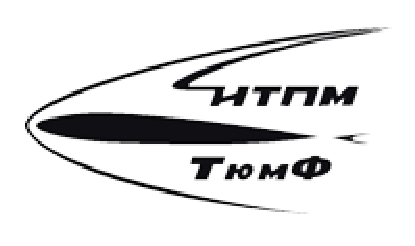
\includegraphics[width=0.1\linewidth]{LOGO_2.EPS}}

\institute[ТюмФ ИТПМ СО РАН]{Тюменский филиал Института теоретической и прикладной механики\\ им. С. А. Христиановича СО РАН, г. Тюмень}

%\date{6 октября 2015 г.}

\begin{document}

\lstset{ %
    language=[ANSI]C++,                 % выбор языка для подсветки (здесь это С++)
    keywordstyle=\color{blue},
    commentstyle=\color{gray},
    basicstyle=\scriptsize,
%basicstyle=\small\sffamily, % размер и начертание шрифта для подсветки кода
    numbers=left,               % где поставить нумерацию строк (слева\справа)
    numberstyle=\tiny,           % размер шрифта для номеров строк
%stepnumber=1,                   % размер шага между двумя номерами строк
    numbersep=4pt,                % как далеко отстоят номера строк от подсвечиваемого кода
%backgroundcolor=\color{white}, % цвет фона подсветки - используем \usepackage{color}
    showspaces=false,            % показывать или нет пробелы специальными отступами
    showstringspaces=false,      % показывать или нет пробелы в строках
    showtabs=false,             % показывать или нет табуляцию в строках
    frame=single,              % рисовать рамку вокруг кода
%tabsize=2,                 % размер табуляции по умолчанию равен 2 пробелам
    captionpos=t,              % позиция заголовка вверху [t] или внизу [b] 
    breaklines=true,           % автоматически переносить строки (да\нет)
    breakatwhitespace=true, % переносить строки только если есть пробел
    escapeinside={\%*}{*)}   % если нужно добавить комментарии в коде
}

%SLIDE #
\begin{frame}

    \transdissolve[duration=0.1]
    \titlepage

\end{frame}

%SLIDE #
\begin{frame}{}

    \transdissolve[duration=0.1]
    \justifying
    \large

    \[
        u_{t} + a u_{x} = 0
    \]

    \begin{columns}
        \begin{column}[T]{0.5\textwidth}
            \begin{center}
                \textbf{Явный метод Эйлера}
            \end{center}

            \[
                \frac{u^{n + 1}_{i} - u^{n}_{i}}{\triangle t} + a \frac{u^{n}_{i} - u^{n}_{i - 1}}{\triangle x} = 0
            \]
        \end{column}
        \begin{column}[T]{0.5\textwidth}
            \begin{center}
                \textbf{Численное решение}
            \end{center}
            \begin{center}
                 \begin{center}
                    \animategraphics[
                        autoplay,
                        width=\textwidth,
                        controls=on,
                        loop
                    ]{50}{./tests/eps/explicitEulerMethod/explicitEulerMethod.}{0}{199}
                \end{center}
            \end{center}
        \end{column}
    \end{columns}

\end{frame}

%SLIDE #
\begin{frame}{}

    \transdissolve[duration=0.1]
    \justifying
    \large

    \begin{center}
        \begin{tabular}{|c|c|c|}
            $u_{t} + a u_{x} = 0$
            &
            $\frac{u^{n + 1}_{i} - u^{n}_{i}}{\triangle t} + a \frac{u^{n}_{i} - u^{n}_{i - 1}}{\triangle x} = 0$
            &
            $\frac{u^{n + 1}_{i} - u^{n}_{i}}{\triangle t} + a \frac{u^{n}_{i} - u^{n}_{i - 1}}{\triangle x} = 0$ + ЭВМ
            \\
            $\Downarrow$ & $\Downarrow$ & $\Downarrow$ \\
            $u = u_{e} \left( x, t\right)$ & $u^{n}_{i} = \left( u_{e} \right)^{n}_{i} + \mathit{O} \left( \triangle x \right)$ & $u^{n}_{i} = \left( u_{e} \right)^{n}_{i} + \mathit{O} \left( \triangle x \right) + \varepsilon$ \\
        \end{tabular}
    \end{center}

\end{frame}

%SLIDE #
\begin{frame}{Дифференциальные приближения}

    \transdissolve[duration=0.1]
    \justifying
    \large

    Попробуем оценить невязку между волновым уравнением:

    \[
        u_{t} + a u_{x} = 0,
    \]

    и разностной схемой, аппроксимирующей его:

    \[
        \frac{u^{n + 1}_{i} - u^{n}_{i}}{\triangle t} + a \frac{u^{n}_{i} - u^{n}_{i - 1}}{\triangle x} = 0,
    \]

\end{frame}

%SLIDE #
\begin{frame}{Дифференциальные приближения}

    \transdissolve[duration=0.1]
    \justifying
    \large

    Для   этого   используем   разложение функции $u(x,t)$ в ряд Тейлора в точках $(x_{i - 1}, t_{i})$ и $(x_{i}, t_{i + 1})$:

    \[
        \begin{split}
            &u^{n + 1}_{i} = u^{n}_{i} + u_{t} \triangle t + \frac{u_{tt}}{2} \triangle t^{2} + \frac{u_{ttt}}{6} \triangle t^{3} + O(\triangle t^{4}),\\
            &u^{n}_{i - 1} = u^{n}_{i} - u_{x} \triangle x + \frac{u_{xx}}{2} \triangle x^{2} - \frac{u_{xxx}}{6} \triangle x^{3} + O(\triangle x^{4}).
        \end{split}
    \]

    Теперь подставим эти разложения в исходную схему.\\

\end{frame}

%SLIDE #
\begin{frame}{Дифференциальные приближения}

    \transdissolve[duration=0.1]
    \justifying
    \large

    \[
        \begin{split}
            &\frac{1}{\triangle t} \left( \left[ u^{n}_{i} + u_{t} \triangle t + \frac{u_{tt}}{2} \triangle t^{2} + \frac{u_{ttt}}{6} \triangle t^{3} + \ldots \right] - u^{n}_{i} \right) +\\
            &+ \frac{a}{\triangle x} \left( u^{n}_{i} - \left[ u^{n}_{i} - u_{x} \triangle x + \frac{u_{xx}}{2} \triangle x^{2} - \frac{u_{xxx}}{6} \triangle x^{3} + \ldots \right] \right) = 0.
        \end{split}
    \]

    После преобразований это выражение приводится к виду

    \[
        \underbrace{u_{t} + a u_{x}}_{\mbox{исходное уравнение}} = \underbrace{- \frac{\triangle t}{2} u_{tt} + \frac{a \triangle x}{2} u_{xx} - \frac{\left( \triangle t \right)^{2}}{6} u_{ttt} - \frac{a \left( \triangle x \right)^{2}}{6} u_{xxx} + \ldots}_{\mbox{погрешность аппроксимации}}.
    \]

\end{frame}

%SLIDE #
\begin{frame}{Дифференциальные приближения}

    \transdissolve[duration=0.1]
    \justifying
    \large

    Значение членов, входящих в погрешность аппроксимации, можно лучше понять, если заменить производные по времени производными по пространству. Для этого
выразим производную $u_{tt}$ через производную по $x$.

    \[
        \begin{split}
            &\; \; \underbrace{\partial_{t} \left[ u_{t} + a u_{x} = - \frac{\triangle t}{2} u_{tt} + \frac{a \triangle x}{2} u_{xx} - \frac{\left( \triangle t \right)^{2}}{6} u_{ttt} - \frac{a \left( \triangle x \right)^{2}}{6} u_{xxx} + \ldots \right]}_{+}\\
            &\overbrace{- a \partial_{x} \left[ u_{t} + a u_{x} = - \frac{\triangle t}{2} u_{tt} + \frac{a \triangle x}{2} u_{xx} - \frac{\left( \triangle t \right)^{2}}{6} u_{ttt} - \frac{a \left( \triangle x \right)^{2}}{6} u_{xxx} + \ldots \right]}
        \end{split}
        \Rightarrow
    \]

\end{frame}

%SLIDE #
\begin{frame}{Дифференциальные приближения}

    \transdissolve[duration=0.1]
    \justifying
    \large

    \[
        u_{tt} = a^{2} u_{xx} + \triangle t \left( - \frac{1}{2} u_{ttt} + \frac{a}{2} u_{ttx} + \mathit{O} \left( \triangle t \right) \right) + \triangle x \left( \frac{a}{2} u_{xxt} - \frac{a^{2}}{2} u_{xxx}  + \mathit{O} \left( \triangle x \right) \right).
    \]

    Аналогично можно получить следующие выражения для производных $u_{ttt}$, $u_{ttx}$, $u_{xxt}$:

    \[
        u_{ttt} = - c^{3} u_{xxx} + \mathit{O} \left( \triangle t, \triangle x \right),
    \]

    \[
        u_{ttx} = c^{2} u_{xxx} + \mathit{O} \left( \triangle t, \triangle x \right),
    \]

    \[
        u_{xxt} = - c u_{xxx} + \mathit{O} \left( \triangle t, \triangle x \right).
    \]

\end{frame}

%SLIDE #
\begin{frame}{Дифференциальные приближения}

    \transdissolve[duration=0.1]
    \justifying
    \large

    Заменим старшие производные по времени и преобразуем выражение к следующему виду:

    \[
        \begin{split}
            &u_{t} + a u_{x} = \frac{a \triangle x}{2} (1 - \sigma) \boxed{u_{xx}} - \frac{a \triangle x^{2}}{6} (2 \sigma^{2} - 3 \sigma + 1) \boxed{u_{xxx}} +\\
            & + O(\triangle x^{3}, \triangle x^{2} \triangle t, \triangle x \triangle t^{2}, \triangle t^{3}).
        \end{split}
    \]

    Уравнение, аналогичное этому, называют \textbf{дифференциальным приближением} или \textbf{модифицированным уравнением} для разностной схемы.\\

    При использовании метода конечных разностей решается на самом деле модифицированное уравнение, а не исходное уравнение в частных производных.

\end{frame}

%%SLIDE #
%\begin{frame}{Дифференциальные приближения}
%
%    \transdissolve[duration=0.1]
%    \justifying
%    \large
%
%    В левой части последнего равенства записано исходное волновое уравнение, а в правой -- погрешность аппроксимации, которая обычно отлична от нуля.\\
%
%    Таким образом, при использовании метода конечных разностей \textbf{решается} на самом деле \textbf{модифицированное уравнение}, а не исходное уравнение в частных производ производных.\\
%
%\end{frame}

%SLIDE #
\begin{frame}{Особенности распространения линейных волн}

    \transdissolve[duration=0.1]
    \justifying
    \large

    Рассмотрим далее общие свойства линейных волн, распространяющихся в одномерном пространстве. В этом случае независимыми переменными являются $t$ и $x$. Волновая система может описываться одной или более зависимыми переменными; рассмотрим пока одну переменную и обозначим ее $u$.\\

    (Иногда употребляют оборот волны с диссипацией и дисперсией -- с точки зрения физики это не верно)

\end{frame}

%SLIDE #
\begin{frame}{Фаза и фазовая скорость}

    \transdissolve[duration=0.1]
    \justifying
    \large

    Рассмотрим волновое изменение зависимой переменной $u \left( x, t \right)$ в виде:

    \[
        u \left( x, t \right) = u_{0} \operatorname{Re} \left\lbrace e^{i \theta} \right\rbrace = u_{0} \cos \left( \theta \right) .
    \]

    $\theta$ -- фаза, линейная по независимым переменным

    \[
        \theta = k x - \omega t + \alpha,
    \]

    $k$ -- волновое число, $\omega$ -- круговая частота.

    Фаза будет оставаться постоянной для наблюдателя, который движется со скоростью

    \[
        \frac{d x}{d t} = \frac{\omega}{k} = c.
    \]

    Действительно

    \[
        \frac{d \theta}{d t} = \frac{\partial \theta}{\partial t} + \frac{d x}{d t} \frac{\partial \theta}{\partial x} = - \omega + \frac{\omega}{k} k = 0.
    \]

\end{frame}

%SLIDE #
\begin{frame}{Дисперсионное соотношение}

    \transdissolve[duration=0.1]
    \justifying
    \large

    В общем случае для распространяющихся волн существует функциональное соотношение $f \left( \omega, k \right)$, связывающее частоту и волновое число. Обычно это соотношение имеет вид зависимости частоты от волнового числа $k$:

    \[
        \omega = W \left( k \right).
    \]

    Соотношение такого типа обычно называют дисперсионным соотношением или уравнением.

    Тогда \textbf{фазовая скорость} также зависит от волнового числа:

    \[
        c = \frac{\omega}{k} = \frac{W \left( k \right)}{k}.
    \]

    В случае, когда фазовая скорость не зависит от волнового числа (или от частоты), говорят, что волна распространяется без дисперсии. В таком случае функция $W$ имеет простой вид:

    \[
        W \left( k \right) = c k.
    \]

\end{frame}

%SLIDE #
\begin{frame}{Интеграл Фурье}

    \transdissolve[duration=0.1]
    \justifying
    \large

    Если начальное распределение $u \left( x, 0 \right)$ не гармонично, то его можно представить с помощью интеграла Фурье как суперпозицию синусоидальных функций.

    \[
        u \left( x, 0 \right) = \frac{1}{2 \pi} \int\limits_{-\infty}^{\infty} \bar{u} \left( p, 0 \right) e^{i p x} dp ,
    \]

    \[
        \bar{u} \left( p, 0 \right) = \int\limits_{-\infty}^{\infty} \bar{u} \left( x, 0 \right) e^{- i p x} dx .
    \]

\end{frame}

%SLIDE #
\begin{frame}{Дисперсия}

    \transdissolve[duration=0.1]
    \justifying
    \large

    Поскольку система предполагается линейной, каждая из гармонических компонент изменяется как $e^{i \theta}$ c частотой $W \left( k \right) = c k$. Полное решение в любой последующий момент времени $t$ может быть получено путем обратного преобразования Фурье.\\

    В бездисперсионном случае этот процесс вновь приводит к начальному распределению, смещенному на расстояние $c t$. То есть, решение можно выразить в виде

    \[
        u \left( x, t \right) = u \left( x - c t, 0 \right).
    \]

Если же волна распространяется с дисперсией, то рассуждения теряют силу. В этом случае каждая компонента Фурье распространяется со своей скоростью.

\end{frame}

%SLIDE #
\begin{frame}{Групповая скорость}

    \transdissolve[duration=0.1]
    \justifying
    \large

    Производная от правой части дисперсионного соотношения имеет размерность скорости

    \[
        C \left( k \right) = \frac{d W}{d k}.
    \]

    Это величина называется \textbf{групповой скорость}.

\end{frame}

%SLIDE #
\begin{frame}{Интерпретация групповой скорости}

    \transdissolve[duration=0.1]
    \justifying
    \large

    Выберем некоторое значение $k$ и соответствующее ему значение $\omega = W \left( k \right)$ как исходные величины и допустим, что кволновому числу добавляется малое возмущение $\pm \triangle k$. Соответствующее возмущенное значение частоты может быть аппроксимировано первыми двумя членами ряда Тейлора:

    \[
        \omega + \triangle \omega = W \left( k + \triangle k \right) \approx \omega + C \triangle k .
    \]

    \[
        \omega - \triangle \omega = W \left( k - \triangle k \right) \approx \omega - C \triangle k .
    \]

    Соответствующие фазы

    \[
        \theta_{+} = \left( k + \triangle k \right) x - \left( \omega + \triangle \omega \right) t = \theta + \triangle k \left( x - C t \right) .
    \]

    \[
        \theta_{-} = \left( k - \triangle k \right) x - \left( \omega - \triangle \omega \right) t = \theta - \triangle k \left( x - C t \right) .
    \]

\end{frame}

\begin{frame}{Интерпретация групповой скорости}

    \transdissolve[duration=0.1]
    \justifying
    \large

    Решение, соответствующее этим двум фазам

    \[
        \begin{split}
            u \left( x, t \right) & = u_{+} \left( x, t \right) + u_{-} \left( x, t \right) = u_{0} \left( \cos \left( \theta_{+} \right) + \cos \left( \theta_{-} \right) \right) = \\
            & = u_{0} \left( \cos \left( \theta + \triangle k \left( x - C t \right) \right) + \cos \left( \theta - \triangle k \left( x - C t \right) \right) \right) = \\
            & = 2 u_{0} \cos \left( \theta \right) \cos \left( \triangle k \left( x - C t \right) \right).
        \end{split}
    \]

    Его можно рассматривать как волну с исходными волновым числом и частотой, модулированную по амплитуде множителем $\cos \left( \triangle k \left( x - C t \right) \right)$. \\

    Другими словами, происходят биения, соответствующие медленным изменениям амплитуды. Колебания ограничены двумя кривыми

    \[
        2 u_{0} \cos \left( \triangle k \left( x - C t \right) \right),
    \]

    которые являются огибающими решения.

%    \begin{center}
%    \begin{animateinline}[controls]{10}
%    \multiframe{180}{iIndex=0+1}{
%        \begin{tikzpicture}
%        \begin{axis}[
%           title=Solution,
%           xlabel={$x$},
%           ylabel={$u \left( x, t \right)$},
%           minor tick num=0,
%           height=0.4\paperheight, 
%           width=0.6\paperwidth,
%           xmin=0,
%           xmax=2*pi,
%           ymin=-1.1,
%           ymax=1.1
%        ]
%        \addplot[
%            blue,
%            very thick,
%            domain=0:2*pi,
%            %samples=50
%        ] {cos(deg(x) - \iIndex)};
%        \addplot[
%            red,
%            very thick,
%            domain=0:2*pi,
%            %samples=50
%        ] {-cos(deg(x) - \iIndex)};
%        \addplot[
%            black,
%            very thick,
%            domain=0:2*pi,
%            samples=200
%        ] {cos(deg(x) - \iIndex)*cos(deg(10*x))};
%        \end{axis}
%        \end{tikzpicture}
%    }
%    \end{animateinline}
%    \end{center}

\end{frame}

\begin{frame}{Интерпретация групповой скорости}

    \transdissolve[duration=0.1]
    \justifying
    \large

    \begin{center}
        \animategraphics[
        width=\textwidth,
        controls=off, loop
        ]{50}{./pic/groupVelocityInterpretation1/fig.}{0}{360}
    \end{center}

    Огибающая движется в пространстве со скоростью $C$. Каждый участок огибающей длиной $\pi/\triangle k$ можно интерпретировать как группу (пакет) волн, а скорость $C$ -- как скорость этой группы. \\

\end{frame}

\begin{frame}{Интерпретация групповой скорости}

    \transdissolve[duration=0.1]
    \justifying
    \large

    \begin{center}
        \animategraphics[
        width=\textwidth,
        controls=off, loop
        ]{50}{./pic/groupVelocityInterpretation2/fig.}{0}{360}
    \end{center}

    \begin{center}
        \animategraphics[
        width=\textwidth,
        controls=off, loop
        ]{50}{./pic/groupVelocityInterpretation3/fig.}{0}{360}
    \end{center}

    В дисперсионном случае групповая скорость отличается от фазовой и может быть как больше, так и меньше фазовой скорости (и даже иметь обратный знак).

\end{frame}

\begin{frame}{Пример №1}

    \transdissolve[duration=0.1]
    \justifying
    \large

    \[
        \boxed{
            \begin{split}
                &u \left( x, t \right) = u_{0} e^{i \left( \omega t - k x \right)} \\
                &u_{t} = i \omega u \\
                &u_{x} = - i k u
            \end{split}
        }
        \Rightarrow
        \boxed{
            u_{t} + a u_{x} = 0
        };
    \]

    \[
        i \omega - a i k = 0;
    \]

    \[
        \omega = W \left( k \right) = a k;
    \]

    \[
        \frac{\omega}{k} = \frac{d W}{d k} = a.
    \]

    \begin{center}
        Точное решение -- волна без дисперсии.
    \end{center}

\end{frame}

%SLIDE #
\begin{frame}{Пример №2}

    \transdissolve[duration=0.1]
    \justifying
    \large

    \[
        \boxed{
            \begin{split}
                &u \left( x, t \right) = u_{0} e^{i \left( \omega t - k x \right)} \\
                &u_{t} = i \omega u \\
                &u_{x} = - i k u \\
                &u_{xx} = - k^{2} u
            \end{split}
        }
        \Rightarrow
        \boxed{
            u_{t} + a u_{x} = \mu u_{xx}
        };
    \]

    \[
        i \omega - i a k = - \mu k^{2}
        \Rightarrow
        \omega = W \left( k \right) = a k + \boxed{i \mu k^{2}};
    \]

    \[
        c = \frac{\omega}{k} = a + \boxed{i \mu k}, \; C = \frac{d W}{d k} = a + \boxed{2 i \mu k};
    \]

\end{frame}

%SLIDE #
\begin{frame}{Пример №2}

    \transdissolve[duration=0.1]
    \justifying
    \large

    \[
         \omega = a k + i \mu k^{2} \Rightarrow u \left( x, t \right) = u_{0} e^{i \left( \omega t - k x \right)};
    \]

    \[
        u \left( x, t \right) = u_{0} e^{i \left( \left( a k + i \mu k^{2} \right) t - k x \right)} = e^{- \mu k^{2} t} e^{i \left( a k t - k x \right)} = e^{\operatorname{\mathbb{I}m}\{\omega\} t} e^{i \left( \operatorname{\mathbb{R}e}\{\omega\} t - k x \right)}.
    \]

    \[
        \operatorname{\mathbb{I}m}\{\omega\} = \beta \: \mbox{-- коэффициент затухания}.
    \]

    \begin{center}
        Точное решение -- затухающая волна без дисперсии.
    \end{center}

\end{frame}

%SLIDE #
\begin{frame}{Пример №3. Уравнение КдВ}

    \transdissolve[duration=0.1]
    \justifying
    \large

    \[
        \boxed{
            \begin{split}
                &u \left( x, t \right) = u_{0} e^{i \left( \omega t - k x \right)} \\
                &u_{t} = i \omega u \\
                &u_{x} = - i k u \\
                &u_{xxx} = i k^{2} u
            \end{split}
        }
        \Rightarrow
        \boxed{
            u_{t} + a u_{x} + b u_{xxx} = 0
        };
    \]

    \[
        i \omega - i a k + i b k^{3} = 0
        \Rightarrow
        \omega = W \left( k \right) = a k - \boxed{b k^{3}};
    \]

    \[
        c = \frac{\omega}{k} = a - \boxed{ b k^{2}}, \; C = \frac{d W}{d k} = a - \boxed{3 b k^{2}};
    \]

    \begin{center}
        Точное решение -- волна с дисперсией.
    \end{center}

\end{frame}

%SLIDE #
\begin{frame}{}

    \transdissolve[duration=0.1]
    \justifying
    \large

    \begin{center}
        \begin{tabular}{|c|c|c|}
            $u_{t} + a u_{x} = 0$
            &
            $u_{t} + a u_{x} = \boxed{\mu u_{xx}}$
            &
            $u_{t} + a u_{x} + \boxed{b u_{xxx}} = 0$
            \\
            $\Downarrow$ & $\Downarrow$ & $\Downarrow$
            \\
            $
                W \left( k \right) = a k
            $
            &
            $
                W \left( k \right) = a k + \boxed{i \mu k^{2}}
            $
            &
            $
                W \left( k \right) = a k - \boxed{b k^{3}}
            $
            \\
            $c = a$
            &
            $c = a + \boxed{i \mu k}$
            &
            $c = a - \boxed{ b k^{2}}$
            \\
            $C = a$
            &
            $C = a + \boxed{2 i \mu k}$
            &
            $C = a - \boxed{3 b k^{2}}$
            \\
            $\beta = 0$
            &
            $\beta = \mu k^{2}$
            &
            $\beta = 0$
            \\
        \end{tabular}
    \end{center}

\end{frame}

%SLIDE #
\begin{frame}{}

    \transdissolve[duration=0.1]
    \justifying
    \large

%    \[
%        u_{t} + a u_{x} = 0
%    \]

%    \vspace{-5pt}

    \begin{columns}
        \begin{column}[T]{0.5\textwidth}
            \begin{center}
                \textbf{Явный метод Эйлера}
            \end{center}
            \[
                \frac{u^{n + 1}_{i} - u^{n}_{i}}{\triangle t} + a \frac{u^{n}_{i} - u^{n}_{i - 1}}{\triangle x} = 0
            \]
            \begin{center}
                \textbf{Дифф. приближение}
            \end{center}
            \[
                \begin{split}
                    &u_{t} + a u_{x} =\\
                    &= \frac{a \triangle x}{2} (1 - \sigma) \boxed{u_{xx}} -\\
                    &\frac{a \triangle x^{2}}{6} (2 \sigma^{2} - 3 \sigma + 1) \boxed{u_{xxx}} + \ldots.
                \end{split}
            \]
        \end{column}
        \begin{column}[T]{0.5\textwidth}
            \begin{center}
                \textbf{Численное решение}
            \end{center}
            \begin{center}
                 \begin{center}
                    \animategraphics[
                        autoplay,
                        width=\textwidth,
                        controls=on,
                        loop
                    ]{50}{./tests/eps/explicitEulerMethod/explicitEulerMethod.}{0}{199}
                \end{center}
            \end{center}
        \end{column}
    \end{columns}

\end{frame}

%%SLIDE #
%\begin{frame}{Численное решение (явный метод Эйлера)}
%
%    \transdissolve[duration=0.1]
%    \justifying
%    \large
%    
%    %ANIMATION #
%    \begin{figure}[h]
%        \center{\animategraphics[autoplay, controls=true, width=0.6\linewidth]{50}{tests/eps/explicitEulerMethod/explicitEulerMethod.}{0}{199}}
%    \end{figure}
%
%\end{frame}

%%SLIDE #
%\begin{frame}{Численное решение (неявный метод Эйлера)}
%
%    \transdissolve[duration=0.1]
%    \justifying
%    \large
%
%    %ANIMATION #
%    \begin{figure}[h]
%        \center{\animategraphics[autoplay, controls=true, width=0.6\linewidth]{50}{tests/eps/implicitEulerMethod/implicitEulerMethod.}{0}{199}}
%    \end{figure}
%
%\end{frame}

%SLIDE #
\begin{frame}{}

    \transdissolve[duration=0.1]
    \justifying
    \large

%    \[
%        u_{t} + a u_{x} = 0
%    \]

%    \vspace{-5pt}

    \begin{columns}
        \begin{column}[T]{0.5\textwidth}
            \begin{center}
                \textbf{Схема Лакса [Lax, 1954]}
            \end{center}
            \[
                \frac{u^{n + 1}_{i} - (u^{n}_{i+1} + u^{n}_{i-1}) / 2}{\triangle t} + a \frac{u^{n}_{i + 1} - u^{n}_{i - 1}}{2 \triangle x} = 0
            \]
            \begin{center}
                \textbf{Дифф. приближение}
            \end{center}
            \[
                \begin{split}
                    &u_{t} + a u_{x} =\\
                    &= \frac{a \triangle x}{2} \left( \frac{1}{\sigma}- \sigma \right) \boxed{u_{xx}} +\\
                    &+ \frac{a \triangle x^{2}}{3} (1 - \sigma^{2}) \boxed{u_{xxx}} + \ldots
                \end{split}
            \]
        \end{column}
        \begin{column}[T]{0.5\textwidth}
            \begin{center}
                \textbf{Численное решение}
            \end{center}
            \begin{center}
                 \begin{center}
                    \animategraphics[
                        autoplay,
                        width=\textwidth,
                        controls=on,
                        loop
                    ]{50}{./tests/eps/LaxScheme/LaxScheme.}{0}{199}
                \end{center}
            \end{center}
        \end{column}
    \end{columns}

\end{frame}

%%SLIDE #
%\begin{frame}{Схема Лакса}
%
%    \transdissolve[duration=0.1]
%    \justifying
%    \large
%
%    \[
%        \begin{split}
%            &u_{t} + a u_{x} = 0 , \\
%            &\frac{u^{n + 1}_{i} - (u^{n}_{i+1} + u^{n}_{i-1}) / 2}{\triangle t} + a \frac{u^{n}_{i + 1} - u^{n}_{i - 1}}{2 \triangle x} = 0 .
%        \end{split}
%    \]
%
%    Дифференциальное приближение для схемы Лакса имеет вид:
%
%    \[
%        u_{t} + a u_{x} = \frac{a \triangle x}{2} \left( \frac{1}{\sigma} - \sigma \right) u_{xx} + \frac{a \triangle x^{2}}{3} (1 - \sigma^{2}) u_{xxx} + ...
%    \]
%
%\end{frame}
%
%%SLIDE #
%\begin{frame}{Численное решение (Схема Лакса)}
%
%    \transdissolve[duration=0.1]
%    \justifying
%    \large
%
%    %ANIMATION #
%    \begin{figure}[h]
%        \center{\animategraphics[autoplay, controls=true, width=0.6\linewidth]{50}{tests/eps/LaxScheme/LaxScheme.}{0}{199}}
%    \end{figure}
%
%\end{frame}

%SLIDE #
\begin{frame}{}

    \transdissolve[duration=0.1]
    \justifying
    \large

%    \[
%        u_{t} + a u_{x} = 0
%    \]

%    \vspace{-5pt}

    \begin{columns}
        \begin{column}[T]{0.5\textwidth}
            \begin{center}
                \textbf{Метод с перешагиванием (метод «чехарда»)}
            \end{center}
            \[
                \frac{u^{n + 1}_{i} - u^{n - 1}_{i}}{2 \triangle t} + a \frac{u^{n}_{i + 1} - u^{n}_{i - 1}}{2 \triangle x} = 0
            \]
            \begin{center}
                \textbf{Дифф. приближение}
            \end{center}
            \[
                \begin{split}
                    &u_{t} + a u_{x} =\\
                    &= \frac{a \triangle x^{2}}{6} \left( \sigma^{2} - 1 \right) \boxed{u_{xxx}} +\\
                    &- \frac{a \triangle x^{4}}{120} (9 \sigma^{4} - 10 \sigma^{2} + 1) \boxed{u_{xxxxx}} + \ldots
                \end{split}
            \]
        \end{column}
        \begin{column}[T]{0.5\textwidth}
            \begin{center}
                \textbf{Численное решение}
            \end{center}
            \begin{center}
                 \begin{center}
                    \animategraphics[
                        autoplay,
                        width=\textwidth,
                        controls=on,
                        loop
                    ]{50}{./tests/eps/leapfrogMethod/leapfrogMethod.}{0}{199}
                \end{center}
            \end{center}
        \end{column}
    \end{columns}

\end{frame}

%%SLIDE #
%\begin{frame}{Метод с перешагиванием (метод «чехарда»)}
%
%    \transdissolve[duration=0.1]
%    \justifying
%    \large
%
%    \[
%        \begin{split}
%            &u_{t} + a u_{x} = 0 , \\
%            &\frac{u^{n + 1}_{i} - u^{n - 1}_{i}}{2 \triangle t} + a \frac{u^{n}_{i + 1} - u^{n}_{i - 1}}{2 \triangle x} = 0 .
%        \end{split}
%    \]
%
%    Дифференциальное приближение для метода «чехарда» имеет вид:
%
%    \[
%        u_{t} + a u_{x} = \frac{a \triangle x^{2}}{6} \left( \sigma^{2} - 1 \right) u_{xxx} - \frac{a \triangle x^{4}}{120} (9 \sigma^{4} - 10 \sigma^{2} + 1) u_{xxxxx} + ...
%    \]
%
%\end{frame}
%
%%SLIDE #
%\begin{frame}{Численное решение (метод «чехарда»)}
%
%    \transdissolve[duration=0.1]
%    \justifying
%    \large
%
%    %ANIMATION #
%    \begin{figure}[h]
%        \center{\animategraphics[autoplay, controls=true, width=0.6\linewidth]{50}{tests/eps/leapfrogMethod/leapfrogMethod.}{0}{199}}
%    \end{figure}
%
%\end{frame}

%SLIDE #
\begin{frame}{}

    \transdissolve[duration=0.1]
    \justifying
    \large

%    \[
%        u_{t} + a u_{x} = 0
%    \]

%    \vspace{-5pt}

    \begin{columns}
        \begin{column}[T]{0.5\textwidth}
            \begin{center}
                \textbf{Метод Лакса -- Вендроффа [Lax, Wendroff, 1960]}
            \end{center}
            \[
                \begin{split}
                    &u^{n + 1}_{i} = u^{n}_{i} - \frac{a \triangle t}{2 \triangle x} (u^{n}_{i + 1} - u^{n}_{i - 1}) + \\
                    & + \frac{a^{2} \triangle t^{2}}{2 \triangle x^{2}} (u^{n}_{i + 1} - 2 u^{n}_{i} + u^{n}_{i - 1})
                \end{split}
            \]
            \begin{center}
                \textbf{Дифф. приближение}
            \end{center}
            \[
                \begin{split}
                    &u_{t} + a u_{x} =\\
                    &= - \frac{a \triangle x^{2}}{6} \left( 1 - \sigma^{2} \right) \boxed{u_{xxx}}\\
                    &- \frac{a \triangle x^{3}}{8} \sigma (1 - \sigma^{2}) \boxed{u_{xxxx}} + \ldots
                \end{split}
            \]
        \end{column}
        \begin{column}[T]{0.5\textwidth}
            \begin{center}
                \textbf{Численное решение}
            \end{center}
            \begin{center}
                 \begin{center}
                    \animategraphics[
                        autoplay,
                        width=\textwidth,
                        controls=on,
                        loop
                    ]{50}{./tests/eps/LaxWendroffMethod/LaxWendroffMethod.}{0}{199}
                \end{center}
            \end{center}
        \end{column}
    \end{columns}

\end{frame}

%%SLIDE #
%\begin{frame}{Метод Лакса -- Вендроффа}
%
%    \transdissolve[duration=0.1]
%    \justifying
%    \large
%
%    \[
%        \begin{split}
%            &u_{t} + a u_{x} = 0 , \\
%            &u^{n + 1}_{i} = u^{n}_{i} - \frac{a \triangle t}{2 \triangle x} (u^{n}_{i + 1} - u^{n}_{i - 1}) + \\
%            & + \frac{a^{2} \triangle t^{2}}{2 \triangle x^{2}} (u^{n}_{i + 1} - 2 u^{n}_{i} + u^{n}_{i - 1}) .
%        \end{split}
%    \]
%
%    Дифференциальное приближение для метода Лакса -- Вендроффа имеет вид:
%
%    \[
%        u_{t} + a u_{x} = - \frac{a \triangle x^{2}}{6} \left( 1 - \sigma^{2} \right) u_{xxx} - \frac{a \triangle x^{3}}{8} \sigma (1 - \sigma^{2}) u_{xxxx} + ...
%    \]
%
%\end{frame}
%
%%SLIDE #?
%\begin{frame}{Численное решение (одношаговый метод Лакса -- Вендроффа)}
%
%    \transdissolve[duration=0.1]
%    \justifying
%    \large
%
%    %ANIMATION #
%    \begin{figure}[h]
%        \center{\animategraphics[autoplay, controls=true, width=0.5\linewidth]{50}{tests/eps/LaxWendroffMethod/LaxWendroffMethod.}{0}{199}}
%    \end{figure}
%
%\end{frame}
%
%%SLIDE #
%\begin{frame}{Численное решение (двухшаговый метод Лакса -- Вендроффа)}
%
%    \transdissolve[duration=0.1]
%    \justifying
%    \large
%
%    %ANIMATION #
%    \begin{figure}[h]
%        \center{\animategraphics[autoplay, controls=true, width=0.5\linewidth]{50}{tests/eps/twoStepLaxWendroffMethod/twoStepLaxWendroffMethod.}{0}{199}}
%    \end{figure}
%
%\end{frame}

%SLIDE #
\begin{frame}{}

    \transdissolve[duration=0.1]
    \justifying
    \large

%    \[
%        u_{t} + a u_{x} = 0
%    \]

    \vspace{-15pt}

    \begin{columns}
        \begin{column}[T]{0.5\textwidth}
            \begin{center}
                \textbf{Метод Мак - Кормака [MacCormack, 1969] (разности против потока [Warming, Beam, 1975])}
            \end{center}
            \vspace{-10pt}
            \[
                \begin{split}
                    &\bar{u}^{n + 1}_{i} = u^{n}_{i} - \frac{a \triangle t}{\triangle x} (u^{n}_{i} - u^{n}_{i - 1}) , \\
                    &u^{n + 1}_{i} = \left[ u^{n}_{i} + \bar{u}^{n + 1}_{i} - \frac{a \triangle t}{\triangle x} (\bar{u}^{n + 1}_{i} - \bar{u}^{n + 1}_{i - 1}) \right. \\
                    &\left. - \frac{a \triangle t}{2 \triangle x} (u^{n}_{i} - 2 u^{n}_{i - 1} + u^{n}_{i - 2}) \right]
                \end{split}
            \]
            \vspace{-15pt}
            \begin{center}
                \textbf{Дифф. приближение}
            \end{center}
            \vspace{-10pt}
            \[
                \begin{split}
                    &u_{t} + a u_{x} =\\
                    &= \frac{a \triangle x^{2}}{6} (1 - \sigma) (2 - \sigma) \boxed{u_{xxx}} -\\
                    &- \frac{\triangle x^{4}}{8 \triangle t} \sigma (1 - \sigma)^{2} (2 - \sigma) \boxed{u_{xxxx}} + \ldots
                \end{split}
            \]
        \end{column}
        \begin{column}[T]{0.5\textwidth}
            \begin{center}
                \textbf{Численное решение}
            \end{center}
            \begin{center}
                 \begin{center}
                    \animategraphics[
                        autoplay,
                        width=\textwidth,
                        controls=on,
                        loop
                    ]{50}{./tests/eps/MacCormackMethodBeamWarmingModification/MacCormackMethodBeamWarmingModification.}{0}{199}
                \end{center}
            \end{center}
        \end{column}
    \end{columns}

\end{frame}

%%SLIDE #
%\begin{frame}{Метод Мак - Кормака (разности против потока)}
%
%    \transdissolve[duration=0.1]
%    \justifying
%    \large
%
%    \[
%        \begin{split}
%            &u_{t} + a u_{x} = 0 , \\
%            &\bar{u}^{n + 1}_{i} = u^{n}_{i} - \frac{a \triangle t}{\triangle x} (u^{n}_{i} - u^{n}_{i - 1}) , \\
%            &u^{n + 1}_{i} = \left[ u^{n}_{i} + \bar{u}^{n + 1}_{i} - \frac{a \triangle t}{\triangle x} (\bar{u}^{n + 1}_{i} - \bar{u}^{n + 1}_{i - 1}) \right. \\
%            & \left. - \frac{a \triangle t}{2 \triangle x} (u^{n}_{i} - 2 u^{n}_{i - 1} + u^{n}_{i - 2}) \right] .
%        \end{split}
%    \]
%
%\end{frame}
%
%%SLIDE #
%\begin{frame}{Метод Мак - Кормака (разности против потока)}
%
%    \transdissolve[duration=0.1]
%    \justifying
%    \large
%
%    Дифференциальное приближение для метода Мак - Кормака имеет вид:
%
%    \[
%        \begin{split}
%            &u_{t} + a u_{x} = \frac{a \triangle x^{2}}{6} (1 - \sigma) (2 - \sigma) u_{xxx} - \\
%            & - \frac{\triangle x^{4}}{8 \triangle t} \sigma (1 - \sigma)^{2} (2 - \sigma) u_{xxxx} + ...
%        \end{split}
%    \]
%
%\end{frame}
%
%%SLIDE #
%\begin{frame}{Численное решение (метод Мак - Кормака)}
%
%    \transdissolve[duration=0.1]
%    \justifying
%    \large
%
%    %ANIMATION #
%    \begin{figure}[h]
%        \center{\animategraphics[autoplay, controls=true, width=0.6\linewidth]{50}{tests/eps/MacCormackMethod/MacCormackMethod.}{0}{199}}
%    \end{figure}
%
%\end{frame}
%
%%SLIDE #
%\begin{frame}{Численное решение (метод Мак - Кормака с разностями против потока)}
%
%    \transdissolve[duration=0.1]
%    \justifying
%    \large
%
%    %ANIMATION #
%    \begin{figure}[h]
%        \center{\animategraphics[autoplay, controls=true, width=0.5\linewidth]{50}{tests/eps/MacCormackMethodBeamWarmingModification/MacCormackMethodBeamWarmingModification.}{0}{199}}
%    \end{figure}
%
%\end{frame}

%%SLIDE #
%\begin{frame}{Диссипация и дисперсия численного решения}
%
%    \transdissolve[duration=0.1]
%    \justifying
%    \large
%
%    Определим диссипацию и диспесиию для дифференциального волнового уравнения. Возьмем решение в виде:
%
%    \[
%        u(x, t) = u_{0} \exp{(i (\omega t - k x))},
%    \]
%
%    где $\omega = 2 \pi \nu$ -- круговая частота, $k = 2 \pi / \lambda$ -- волновое число.\\
%
%    Подставив это решение в волновое уравнение, получим зависимость $\omega = \omega(k)$, которая называется \textbf{дисперсионным соотношением}.\\
%
%    Если $\omega$ -- комплексное число, волна затухает!
%
%    \[
%        \exp{((- Im \omega) t)} = \exp{(- \gamma t)}.
%    \]
%
%\end{frame}
%
%%SLIDE #
%\begin{frame}{Фазовая и групповая скорость}
%
%    \transdissolve[duration=0.1]
%    \justifying
%    \large
%
%    \textbf{Фазовая скорость} -- это скорость, с которой движется фаза или отдельной гармоники:
%
%    \[
%        \frac{Re \omega}{k} = c_{f}.
%    \]
%
%    \textbf{Групповая скорость} -- это скорость волнового пакета, состоящего из гармонических волн с близкими волновыми числами (Передача энергии осуществляется с групповой скоростью!):
%
%    \[
%        \frac{d}{d k} Re \omega = c_{g}.
%    \]
%
%\end{frame}
%
%%SLIDE #
%\begin{frame}{Дисперсия волн}
%
%    \transdissolve[duration=0.1]
%    \justifying
%    \large
%
%    Если фазовая/групповая скорость зависит от $k$, то гармоники с разными волновыми числами распространяются с разными скоростями. Такое явление называется \textbf{дисперсией}.
%
%\end{frame}
%
%%SLIDE #
%\begin{frame}{Пример №1}
%
%    \transdissolve[duration=0.1]
%    \justifying
%    \large
%
%    \[
%        \frac{\partial^{2} u}{\partial t^{2}} = c^{2} \frac{\partial^{2} u}{\partial x^{2}} \Rightarrow - \omega^{2} = - c^{2} k^{2} \Rightarrow \omega = c k \Rightarrow \frac{Re \omega}{k} = \frac{d}{d k} Re \omega = c.
%    \]
%    
%    Точное решение -- волна без дисперсии и затухания.
%
%\end{frame}
%
%%SLIDE #
%\begin{frame}{Пример №2}
%
%    \transdissolve[duration=0.1]
%    \justifying
%    \large
%
%    \[
%        \frac{\partial u}{\partial t} + c \frac{\partial u}{\partial x} = \mu \frac{\partial^{2} u}{\partial x^{2}} \Rightarrow i \omega - i c k = - \mu k^{2} \Rightarrow \omega(k) = c k + i \mu k^{2}.
%    \]
%    
%    Точное решение -- затухающая недиспергирующая волна.
%
%\end{frame}

%SLIDE #
\begin{frame}{Диссипация и дисперсия сеточного решения}

    \transdissolve[duration=0.1]
    \justifying
    \large

    Анализ диссипации и дисперсии сеточного решения можно проводить на решении

    \[
        u^{n}_{i} = u^{*} e^{i \left( \omega t_{n} - k x_{i} \right)}.
    \]
    
    После подстановки этого решения в разностную схему, получим сеточное дисперсионное соотношение $\omega = W \left( k, \triangle t, \triangle x \right)$.

\end{frame}

%SLIDE #
\begin{frame}{Пример}

    \transdissolve[duration=0.1]
    \justifying
    \large

    Метод с перешагиванием (метод «чехарда»):

    \[
        \boxed{
        \begin{split}
            &u^{n + 1}_{i} = u^{*} e^{i \left( \omega \left( t_{n} + \triangle t \right) - k x_{i} \right)}\\
            &u^{n - 1}_{i} = u^{*} e^{i \left( \omega \left( t_{n} - \triangle t \right) - k x_{i} \right)}\\
            &u^{n}_{i + 1} = u^{*} e^{i \left( \omega t_{n} - k \left( x_{i} + \triangle x \right) \right)}\\
            &u^{n}_{i - 1} = u^{*} e^{i \left( \omega t_{n} - k \left( x_{i} - \triangle x \right) \right)}
        \end{split}
        }
        \Rightarrow
        \frac{u^{n + 1}_{i} - u^{n - 1}_{i}}{2 \triangle t} + a \frac{u^{n}_{i + 1} - u^{n}_{i - 1}}{2 \triangle x};
    \]

    \[
        e^{i \omega \triangle t} - e^{- i \omega \triangle t} + \sigma \left( e^{- i k \triangle x} - e^{i k \triangle x} \right)= 0;
    \]

    \[
        \sin{\left( \omega \triangle t \right)} = \sigma \sin{\left( k \triangle x \right)}
        \Rightarrow
        \omega = \frac{1}{\triangle t} \arcsin{\left( \sigma \sin{\left( k \triangle x \right)} \right)};
    \]

    \[
        c = \frac{W}{k} = \frac{1}{k \triangle t} \arcsin{\left( \sigma \sin{\left( k \triangle x \right)} \right)}, \;
        C = \frac{d W}{d k} = a \frac{\cos{\left( k \triangle x \right)}}{\sqrt{1 - \sigma^{2} \sin{\left( k \triangle x \right)}}}.
    \]

\end{frame}

%%SLIDE #
%\begin{frame}{Дак вот оно что!}
%
%    \transdissolve[duration=0.1]
%    \justifying
%    \large
%
%    Теперь можно объяснить возникновение осцилляций в приближенном решении. Любое гладкое решение можно представить в виде ряда Фурье по пространственным гармоникам:
%
%    \[
%        u(x, t) = u_{1}(t) u_{2}(x) \approx u_{1}(t) \sum^{N}_{n = 0} \left( a_{n} \cos \left( \frac{2 \pi n x}{l} \right) + b_{n} \sin \left( \frac{2 \pi n x}{l} \right) \right).
%    \]
%
%    Возникает дисперсия приближенного решения и гармоники с разными значениями $n$ распространяются с разными скоростями. Возникает пространственное разделение этих гармоник, и появляются осцилляции, отсутствующие в точном решении.
%
%\end{frame}

%SLIDE #
\begin{frame}{Заключение}

    \transdissolve[duration=0.1]
    \justifying
    \large

    При численном решении волновых задач возникает затухание и дисперсия сеточного решения, что связано с формой разностных уравнений. Затухание прводит к уменьшению амплитуды, дисперсия -- искажает форму волны.

\end{frame}

\end{document}